\subsection{Q1 v2 配比效应与条件广义标度律}

问题一正式发布版本为 \texttt{chm.q1.v2.0}；清单 SHA256 以前缀
\texttt{c621f7e4} 标识，完整校验值见随结果发布的 \texttt{upstream\_pin.json}。
我们只消费发布的模型系数、特征定义、512 条配方和 A1 主质量映射，不在本节重读原始附件 A。
该模型对 13 个目标域各有 17 个配比主项和 10 个双线性交互项。
以各目标模型自身的正参考预测 $R_k=\widehat L_{A,k}(\boldsymbol p_{\rm ref})$ 定义
\begin{equation}
r_k(\boldsymbol p)=\frac{\widehat L_{A,k}(\boldsymbol p)-R_k}{R_k},
\qquad r_w(\boldsymbol p)=\sum_{k=1}^{13}w_kr_k(\boldsymbol p),\quad
w_k\geq0,\ \sum_kw_k=1.
\end{equation}
这些是 1M A 侧、逐目标 Loss 的相对效应；B7 的 $Q_B$ 是另一个原生质量坐标，不能将 $Q_A$ 代入。
目标权重表示分析政策，不是训练域配比。

在明确的跨来源迁移假设下，我们取可直接调用的条件基准
\begin{equation}
\label{eq:cyj-v7-baseline}
L_{\rm base}(N,D,Q_B,\boldsymbol p;w)
=L_B(N,D,Q_B)\exp\{r_w(\boldsymbol p)\}.
\end{equation}
这约定 B7 曲面对应参考配方，并将 A 侧相对效应放入 B 侧的 log-Loss。
参考点返回 $L_B$，小效应下指数形式与 $1+r_w$ 一阶一致，且在数值有效时保持正 Loss。
这些是模型内部性质，不证明 B 的实际训练配方等于参考点，也不证明 A/B Loss 口径相同。
附件没有两侧在相同 $N,D,Q_B,\boldsymbol p$ 下的成对结果，迁移幅度及规模调制不能被识别。

为检验结论依赖，另设 $a=\lambda(N/1\,\mathrm{B})^{-\eta}$，比较
$L_{\exp}=L_Be^{a r_w}$ 与 $L_{\rm lin}=L_B(1+a r_w)$；后者只在括号正时有效。
式\eqref{eq:cyj-v7-baseline} 固定 $\lambda=1,\eta=0$，只是条件政策，不是从联合数据估出的参数。
敏感性覆盖 $\lambda=0,0.5,0.75,1,1.25,1.5$ 和 $\eta=0,0.1,0.2,0.4$，
并在 $N=0.1,1,10$B 与两种桥接形式上逐项计算；无效线性因子按无效情景记录。
这些情景范围不构成置信区间。

图\ref{fig:cyj-v7-bridge} 展示等权凸包可行候选在三个规模下的指数桥接情景。
它只比较固定配方的条件 Loss；随 $N$ 分离的曲线来自假设中的 $N^{-\eta}$，并非观测到跨规模配比效应。
\begin{figure}[htbp]
\centering
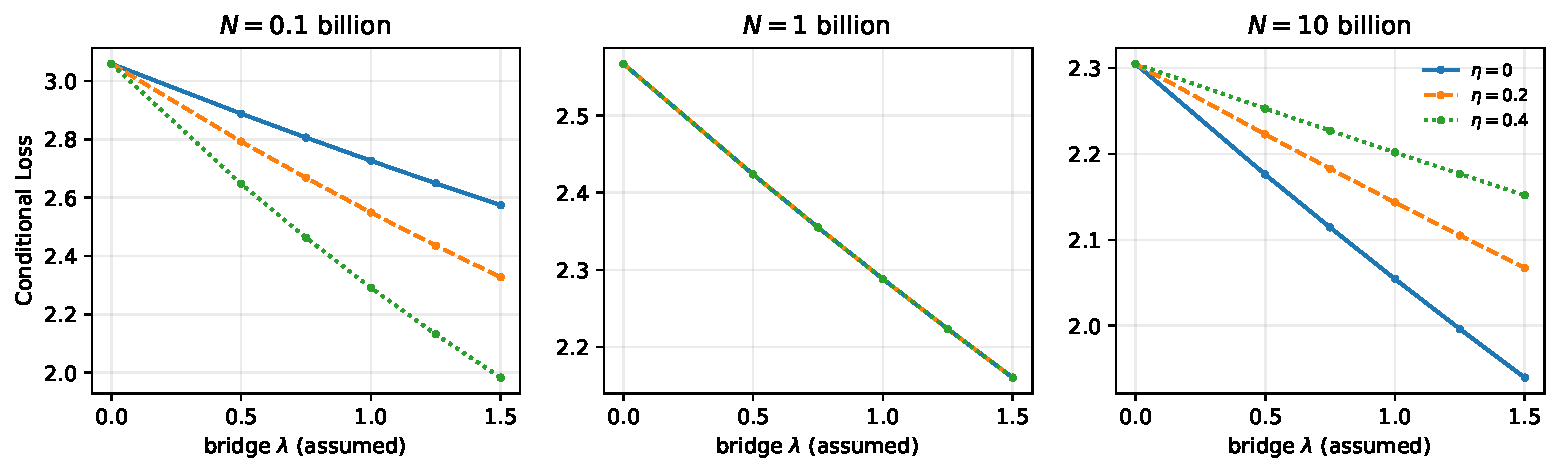
\includegraphics[width=0.96\textwidth]{figures/cyj/q2_v7_bridge_sensitivity.pdf}
\caption{固定配方的条件桥接敏感性；点来自明示网格，非置信区间。}
\label{fig:cyj-v7-bridge}
\end{figure}

\subsection{支持域、质量政策与配比决策}

基础配比域为 A4 归一化 512 条配方的凸包。
CHM 在 13 域等权及两项质量政策下给出数值可行上界和 McCormick 松弛下界，
其间隙在 0.001 相对效应以内，但并非严格区间算术的全局最优证明。
我们逐项复核了权重、分母、模型清单、目标和质量限制。
单目标 arxiv、pile\_cc 的 512 条观测配方做精确枚举；另以同一数值 McCormick 分枝界算法对其连续凸包分别求得小于 0.001 的相对效应间隙。
这两项由 CYJ 扩展求解并核验，不属于 CHM 原四政策签收，也不声称严格全局最优证明。

质量政策只对已映射的 direct 或 direct+near 域计算 A1 评分。
要求质量覆盖比例及映射域条件均值均不低于参考配方；无映射的 11 域保持缺失，不能填零解释为低质。
这是配比可行性约束，不提供 $Q_A\rightarrow Q_B$ 或质量成本函数。
在 $N=1$B、$D=100$B、$Q_B=0.5$ 的固定展示点，B7 Loss 为 2.567397。
等权连续凸包可行候选的 $r_w=-0.115112$，条件 Loss 为 2.288234；
direct 和 direct+near 政策的对应条件 Loss 分别为 2.316137 和 2.330034。
最差目标保护策略最小化 $\max_k r_k$，它不是等权目标；其可行候选等权评估 Loss 为 2.487281。
单目标 arxiv、pile\_cc 的连续凸包可行候选条件 Loss 分别为 1.538707、2.237045；这些值只与各自目标定义比较。
这些数值可由本节结果目录的 \texttt{policy\_solutions.csv}、
\texttt{policy\_details.json} 和 CHM 发布的凸包界表复核，
不是联合 A/B 实测改进。

固定 $N,D,Q_B,w$ 和相同有效可行域，$e^r$ 与 $1+r$ 都严格递增，
故两种桥接的配比排序和最优解集合必然相同。排序一致仅是代数及实现核验，
不能作为跨来源假设正确的经验支持。$\lambda=0$ 时所有可行配方在条件 Loss 上并列。
不同质量政策、权重或联合预算约束则可能改变比较对象，必须逐项注明。
512 条观测配方的等权比较中，两桥接共同有效 512 条、线性无效 0 条，排序完全一致；
绝对 Loss 差的观测最大值为 0.026782，不能将这个样本最大值称为连续凸包上界。

\subsection{边际、弹性和领域间替代}

记 $r=r_w(\boldsymbol p)$。条件基准对 $x\in\{N,D,Q_B\}$ 满足
\begin{equation}
L_x=e^r(L_B)_x,\qquad
\nabla_{\boldsymbol p}L=L\nabla_{\boldsymbol p}r,\qquad
\nabla^2_{\boldsymbol p}L=L\bigl[\nabla^2r+(\nabla r)(\nabla r)^\top\bigr].
\end{equation}
我们报告带符号弹性 $xL_x/L$；固定配比时，$N,D,Q_B$ 的弹性与冻结 B7 完全相同。
配比总和恒为 1，只有保持单纯形和凸包可行的方向才有操作含义。
例如从当前配方向另一条满足相同质量政策的已观测配方移动，
以两配方之差作为方向计算一阶变动和二阶曲率，
并用小步长重新调用 predictor 核对。对两条从同一配比出发的可行方向，
还比较混合方向曲率 $\boldsymbol u^\top H_pL\boldsymbol v$ 与双向有限差分。
指数变换自身引入 $(\nabla r)(\nabla r)^\top$ 曲率，
因此 Q1 的交互系数符号不能直接当作 Q2 的互补或因果作用。
数值与方向可行性见领域转移、曲率两张结果表。
在观测配方集上的连续方向只属于其凸包，不等于新的已观测配方。

固定 $D,\boldsymbol p$，求提升 $Q_B$ 后相同 Loss 所需的 $N'$，
式\eqref{eq:cyj-v7-baseline} 两边的指数因子消去，根与 B7 相同。
只有在 $Q_B+\Delta Q$ 与 $N'$ 均处支持范围、方程存在域内根时报告数值；
无根明确标记。例如在 $N=11$B、$D=100$B、$Q_B=0.5$，提升质量 0.2 的等 Loss 方程在声明的 $N$ 范围内无根。
根、边界与残差见 \texttt{quality\_vs\_scale.csv}。
若配比成本和可行域不随预算变，最优配比集合也不随预算变；
问题三出现配比结构转移需要另有明确的成本或约束耦合，不能由式\eqref{eq:cyj-v7-baseline} 自行推出。

\subsection{验证层级、识别边界与复现}

A6--A11 曾参与 Q1 模型形式比较，不能再次充作未触碰终测；
A12--A15 的估算/外推记录不是真实训练观测。
B7 的留组评价只支持半合成同源条件关系；B6 是 B7 子集，B8 的质量方向与 B7 冲突，
B4/B5 与 B1 的 Loss 坐标尚未证明可比，B10 为估算值。
锚点、桥接排序与导数差分是内部核验。真正检验跨来源迁移，需要相同 tokenizer 和验证目标、
共同的参考及变化配方、受控 $N,D,Q_B$ 的成对重复实验，并事先指定误差与拒绝标准。
现有附件未提供这种检验，故不报告跨源预测误差或联合置信区间。
冻结的 B7 联合候选另有 200 次 $(N,D)$ 簇重抽样参数样本。
固定等权连续凸包配方及桥接因子时，其条件 Loss 的参数样本 2.5\% 与 97.5\% 分位数为 2.279458、2.296272；
这仅传播半合成 B7 的参数变化，不包含 Q1 系数、桥接机制或跨源误差，不能当作联合预测区间。

版本化接口为 \texttt{cyj.ndqp.scenario.v7}，明确声明结果以桥接假设为条件，且尚未经过跨来源实证校准。
固定政策、输入哈希、环境与输出清单存于 Q2 v7 结果目录。
Q2 运行期间的 Python 文件打开审计记录原始 A 为零次；审计文件同时说明覆盖范围与限制。
CHM 的 Q3 消费验收和问题四能力映射是后续独立步骤；本节结论仅限所述假设、支持域和数据角色。

\clearpage
